% =====================================================================
%  Cómo interpretar las gráficas del análisis en frecuencia
%  Compilar con:  pdflatex guia_graficas.tex  (dos pasadas)
%  Las figuras están en figuras/ (las explicativas salen de hacer_figuras.py y las de
%  los ejemplos, de ../analisis_simple/analisis.py).
% =====================================================================
\documentclass[11pt,a4paper]{article}
\usepackage[utf8]{inputenc}
\usepackage[T1]{fontenc}
\usepackage{lmodern}
\usepackage[spanish,es-noshorthands,es-tabla]{babel}
\usepackage{amsmath,amssymb}
\usepackage{icomma}
\usepackage[a4paper,left=2.2cm,right=2.2cm,top=2.3cm,bottom=2.3cm,headheight=14pt]{geometry}
\usepackage{xcolor}
\usepackage{graphicx}
\usepackage{booktabs,array,tabularx}
\usepackage{enumitem}
\usepackage{titlesec}
\usepackage{fancyhdr}
\usepackage{needspace}
\usepackage[most]{tcolorbox}
\usepackage[font=small,labelfont=bf]{caption}
\usepackage[colorlinks=true,linkcolor=azul,urlcolor=azul]{hyperref}

% ---------------------------------------------------------------- colores
\definecolor{azul}{RGB}{31,78,121}
\definecolor{verde}{RGB}{0,115,70}
\definecolor{rojo}{RGB}{185,30,40}
\definecolor{naranja}{RGB}{215,110,0}
\definecolor{gris}{RGB}{95,95,95}

% ---------------------------------------------------------------- títulos
\titleformat{\section}{\Large\bfseries\color{azul}}{\thesection.}{0.5em}{}
\titleformat{\subsection}{\large\bfseries\color{azul}}{\thesubsection}{0.5em}{}
\titlespacing*{\section}{0pt}{14pt plus 3pt}{6pt}
\titlespacing*{\subsection}{0pt}{10pt plus 2pt}{4pt}
\setlength{\parindent}{0pt}
\setlength{\parskip}{4pt plus 1pt}
\setlist{itemsep=1pt,topsep=2pt,parsep=1pt}
\newcommand{\pct}{\ensuremath{\,\mathchar"7025}}
\newcommand{\rads}{\,\mathrm{rad/s}}
\newcommand{\dB}{\,\mathrm{dB}}
\newcommand{\dBdec}{\,\mathrm{dB/dec}}
\newcommand{\wc}{\omega_c}
\newcommand{\wcien}{\omega_{180}}
\newcommand{\MF}{\mathrm{MF}}
\newcommand{\MG}{\mathrm{MG}}
\newcommand{\Mr}{M_r}
\newcommand{\arch}[1]{\texttt{#1}}

\pagestyle{fancy}
\fancyhf{}
\lhead{\small\color{gris}Sistemas de Control}
\rhead{\small\color{gris}Cómo leer las gráficas}
\cfoot{\small\thepage}
\renewcommand{\headrulewidth}{0.4pt}

% ---------------------------------------------------------------- cajas
\tcbset{base/.style={enhanced,breakable,boxrule=0.6pt,arc=2pt,left=6pt,right=6pt,top=4pt,bottom=4pt,
  fonttitle=\bfseries\small,before skip=6pt,after skip=6pt}}
\newtcolorbox{idea}{base,colback=azul!5,colframe=azul,title={Idea clave}}
\newtcolorbox{nota}{base,colback=naranja!5,colframe=naranja,title={Ojo}}
\newtcolorbox{regla}{base,colback=verde!5,colframe=verde,title={Regla práctica}}

% figura centrada con ancho relativo
\newcommand{\fig}[3]{\begin{figure}[htbp]\centering\includegraphics[width=#2\textwidth]{figuras/#1}\caption{#3}\end{figure}}

\begin{document}

% =====================================================================
%  PORTADA
% =====================================================================
\begin{center}
{\LARGE\bfseries\color{azul} Cómo interpretar las gráficas\par}
\vspace{4pt}
{\large Bode, Nyquist, Nichols y respuesta al escalón\par}
\vspace{2pt}
{\small\color{gris} Guía para leer lo que produce \texttt{analisis.py}\par}
\end{center}
\vspace{4pt}

\begin{idea}
Todas las gráficas (menos la respuesta al escalón) son la \emph{misma curva} $L(j\omega)$ dibujada en distintas
coordenadas. La que importa es el punto crítico $L=-1$: ``estar cerca de $-1$'' es tener poco margen, y cada gráfica
te muestra esa distancia de una manera distinta. Si entendés eso, el resto es saber dónde mirar.
\end{idea}

\section{Qué te da el programa y en qué orden mirarlo}

Al correr \texttt{analisis.py} salen un texto en el terminal y hasta cinco figuras. Conviene mirar siempre primero el
\textbf{texto} (tiene los números exactos) y después las figuras (te dicen por qué).

\begin{center}
\small
\begin{tabularx}{\textwidth}{@{}l>{\raggedright\arraybackslash}X>{\raggedright\arraybackslash}X@{}}
\toprule
Figura & Qué muestra & Pregunta que responde\\
\midrule
\arch{1\_bode} & $|L|$ en dB y $\angle L$ en grados contra $\omega$ (log) & ¿De qué tipo es? ¿Dónde cruza? ¿Cuánto MF y MG tengo? \\
\arch{2\_nyquist} & $L(j\omega)$ en el plano complejo, con el $-1$ y el círculo $|L|=1$ & ¿Es estable? ¿Qué tan lejos pasa del $-1$? \\
\arch{3\_nichols} & $\angle L$ (horizontal) contra $|L|$ en dB (vertical), con curvas de $|T|$ constante & ¿Cuánto vale $\Mr$? ¿Cómo mover la curva? \\
\arch{4\_escalon} & Respuesta temporal en lazo cerrado & ¿Cómo se ve en el tiempo? \\
\arch{5\_compensador} & Bode de $G_c(s)$ solo & ¿Qué le hace el compensador al lazo? \\
\bottomrule
\end{tabularx}
\end{center}

En todas las figuras \textcolor{azul}{\textbf{azul}} es el sistema sin compensar y \textcolor{rojo}{\textbf{rojo}} el compensado.
Se usan dos ejemplos para ilustrar: el \textbf{Ejemplo A} (parcial 1: $G=K/(s^3+10s^2+5s)$ con $K=100$ y un atraso) y
el \textbf{Ejemplo B} (un adelanto sobre $10/[s(s+1)(0{,}05s+1)]$).

\section{Todo sale del lazo abierto \texorpdfstring{$L(s)$}{L(s)}}

El programa trabaja con el \textbf{lazo abierto} $L(s)=G_c(s)\,G(s)\,H(s)$ (con $H=1$ si la realimentación es
unitaria). El lazo cerrado es $T(s)=G_cG/(1+G_cGH)$.

El lazo cerrado se vuelve inestable cuando $L$ vale exactamente $-1$ para alguna frecuencia, o sea
\[
|L(j\omega)|=1\ (0\dB)\qquad\text{y}\qquad \angle L(j\omega)=-180^\circ .
\]
Ese único punto se ve en cada gráfica de una forma distinta:

\begin{center}
\small
\begin{tabular}{@{}ll@{}}
\toprule
Gráfica & Dónde está el punto crítico \\
\midrule
Bode & la curva de magnitud toca 0 dB \emph{a la misma frecuencia} en que la fase vale $-180^\circ$ \\
Nyquist & el punto $-1+j0$ \\
Nichols & el punto $(-180^\circ,\ 0\dB)$ \\
\bottomrule
\end{tabular}
\end{center}

Los dos márgenes miden qué tan lejos se pasa del punto crítico:
\begin{itemize}
\item \textbf{Frecuencia de cruce} $\wc$: donde $|L(j\wc)|=1$. \textbf{Margen de fase}: $\MF=180^\circ+\angle L(j\wc)$.
 Es cuánta fase más podría perder el lazo antes de llegar a $-180^\circ$ justo en el cruce.
\item \textbf{Frecuencia de cruce de fase} $\wcien$: donde $\angle L(j\wcien)=-180^\circ$. \textbf{Margen de ganancia}:
 $\MG=1/|L(j\wcien)|$, o en dB, $\MG_{\mathrm{dB}}=-20\log|L(j\wcien)|$. Es por cuánto se puede multiplicar la ganancia
 antes de llegar a inestabilidad.
\end{itemize}
El programa informa $\MG$ en veces y en dB: $\MG=2$ equivale a $6{,}02\dB$ y $\MG=0{,}5$ a $-6{,}02\dB$.

\section{Diagrama de Bode}

\fig{bode_anatomia.png}{0.82}{Anatomía del Bode de $L=4/[s(s+1)(0{,}1s+1)]$ (tipo 1, $K_v=4$): lo que hay que leer en cada zona.}

\subsection{Qué se dibuja}
Arriba, $20\log_{10}|L(j\omega)|$ en dB; abajo, la fase en grados; en ambos el eje horizontal es $\omega$ en escala
logarítmica. Un polo real en $\omega=1/\tau$ baja la pendiente de la magnitud en $20\dBdec$ y la fase en $90^\circ$
(es $-45^\circ$ justo en el quiebre, y casi todo el cambio ocurre en la década anterior y la posterior). Un cero hace lo
contrario. Los polos complejos poco amortiguados dan un pico (resonancia) y una caída de fase abrupta.

\subsection{Cómo leerlo, en orden}
\begin{enumerate}
\item \textbf{La pendiente inicial dice el tipo.} Horizontal: tipo 0; $-20\dBdec$: tipo 1 (un integrador);
 $-40\dBdec$: tipo 2. La fase arranca en $-90^\circ\times$(tipo).
\item \textbf{La altura dice la constante de error.} Tipo 0: la meseta vale $20\log K_p$. Tipo 1: la asíntota de
 $-20\dBdec$ corta 0 dB en $\omega=K_v$ (en la figura, $K_v=4$). Tipo 2: la asíntota de $-40\dBdec$ corta 0 dB en
 $\omega=\sqrt{K_a}$.
\item \textbf{Los cambios de pendiente son los polos y ceros.} Cada quiebre que baja $20\dBdec$ es un polo; cada uno
 que sube, un cero. Sirve para chequear que la función que ingresaste es la que creés.
\item \textbf{$\wc$:} dónde la magnitud cruza 0 dB. Es la medida de velocidad del lazo: el ancho de banda de lazo cerrado
 suele ser entre 1 y 2 veces $\wc$.
\item \textbf{$\MF$:} leer la fase en $\wc$ y ver cuánto falta para $-180^\circ$.
\item \textbf{$\MG$:} leer cuántos dB por debajo de 0 está la magnitud en $\wcien$.
\end{enumerate}

\begin{regla}
\textbf{La pendiente con que se cruza 0 dB.} Para sistemas de fase mínima, una pendiente de $-20\dBdec$ corresponde a
fase cercana a $-90^\circ$, una de $-40\dBdec$ a $-180^\circ$ y una de $-60\dBdec$ a $-270^\circ$. Por eso:
cruzando con $-20\dBdec$ (durante alrededor de una década) el $\MF$ sale holgado; con $-40\dBdec$ es justo y depende de
qué tan lejos esté el siguiente quiebre; con $-60\dBdec$ el lazo cerrado casi seguro es inestable. En la figura, el cruce
cae en el tramo de $-40\dBdec$ y el margen de fase es $18^\circ$: oscilará mucho.
\end{regla}

\subsection{Cuántos margen es suficiente}
Criterios habituales (si el enunciado pide otros, valen esos):
\begin{center}
\small
\begin{tabular}{@{}lll@{}}
\toprule
& Justo / oscilatorio & Bueno \\
\midrule
$\MF$ & menor que $30^\circ$ & entre $45^\circ$ y $60^\circ$ \\
$\MG$ & menor que 6 dB ($\times2$) & entre 8 y 12 dB \\
\bottomrule
\end{tabular}
\end{center}
Un $\MF$ mucho mayor que $60^\circ$ suele significar un sistema lento o con ganancia de más sobrando.

\subsection{Casos que confunden}
\begin{itemize}
\item \textbf{Márgenes negativos.} $\MF<0$ y $\MG<1$ (dB negativos): en un sistema de fase mínima y lazo abierto estable,
 el lazo cerrado es \emph{inestable}. En el Ejemplo A sin compensar: $\MF=-8{,}8^\circ$ y $\MG=0{,}5=-6{,}02\dB$.
\item \textbf{Sin cruce.} Si $|L|$ nunca llega a 0 dB (por ejemplo $1/(s+1)$), no hay $\MF$ y el programa lo avisa;
 si la fase nunca llega a $-180^\circ$, el $\MG$ es infinito (es lo normal en sistemas de primer y segundo orden).
\item \textbf{Varios cruces.} Si la fase cruza $-180^\circ$ más de una vez (sistemas condicionalmente estables) o la
 magnitud cruza 0 dB más de una vez, los márgenes que se informan son los del cruce principal. No te quedes con ellos:
 mirá el Nyquist y la cuenta $Z=N+P$.
\item \textbf{Lazo abierto inestable.} Ahí el criterio se invierte: ver la sección de Nyquist y la sección de trampas.
\end{itemize}

\section{Diagrama de Nyquist}

\fig{nyquist_galeria.png}{1.0}{Seis formas típicas. Línea llena: $\omega>0$; línea rayada: $\omega<0$ (espejo). La cruz roja es el $-1$.
En (a)--(d) $L=K/[s(s+1)(s+2)]$ con $K=1,\,12,\,6$ y $L=2(s+3)/[s(s-1)]$; en (e) y (f), $L=Ke^{-0{,}8s}/[s(s+1)]$ con $K=1$ y $1{,}5$.}

\subsection{Qué se dibuja}
La curva $L(j\omega)$ en el plano complejo (parte real horizontal, parte imaginaria vertical). La línea llena es
$\omega>0$ y la rayada es la imagen espejo ($\omega<0$). Las flechas, cuando hay, apuntan hacia $\omega$ creciente.
En el programa, además, se dibuja el círculo punteado $|L|=1$.

Dos cosas del dibujo que hay que saber:
\begin{itemize}
\item La figura es un \textbf{zoom alrededor de $-1$}; lo que está lejos queda afuera. Si hay integradores, a baja
 frecuencia la curva viene desde el infinito (tipo 1: desde abajo, con una asíntota vertical; tipo 2: desde la izquierda).
\item El \textbf{arco de radio infinito} que cierra el contorno alrededor de los integradores no se dibuja, pero el programa
 sí lo incluye en la cuenta de rodeos.
\end{itemize}

\subsection{El criterio y cómo se lee}
\[
Z = N + P
\]
donde $P$ es la cantidad de polos de $L$ en el semiplano derecho, $N$ es la cantidad de rodeos \emph{en sentido horario}
de la curva completa al punto $-1$, y $Z$ es la cantidad de polos de lazo cerrado en el semiplano derecho. Lazo cerrado
estable $\iff Z=0$. El programa imprime $P$, $N$ y $Z$ y además cuenta las raíces del lazo cerrado como verificación.

\begin{regla}
Con $P=0$ (lo más común) y la curva cruzando el eje real negativo una sola vez: si cruza \textbf{a la derecha} de $-1$
(entre $-1$ y $0$), el lazo es estable; si cruza \textbf{a la izquierda}, inestable; si pasa por $-1$, está en el
límite. El valor del cruce es $-1/\MG$: en la figura (b) cruza en $-2$, o sea $\MG=0{,}5$ ($-6\dB$) y el lazo es inestable
con $N=2$.
\end{regla}

\subsection{Los márgenes en el Nyquist}
\begin{itemize}
\item \textbf{$\MG$:} el punto donde la curva corta el eje real negativo está en $-1/\MG$.
\item \textbf{$\MF$:} se lee donde la curva corta el círculo $|L|=1$; el ángulo entre ese punto y el eje real negativo es el
 $\MF$.
\item \textbf{Robustez:} la distancia mínima de la curva al punto $-1$ es $1/M_s$ (con $M_s=\max|S|$, el pico de la
 función de sensibilidad). Cuanto más lejos pasa de $-1$, más tolera el lazo errores del modelo.
\end{itemize}

\subsection{Panel por panel}
\begin{description}[leftmargin=1.2em,labelindent=0pt]
\item[(a) Estable.] Cruza en $-1/6$: queda lejos del $-1$ ($\MG=6$, unos $15{,}6\dB$). $N=0$.
\item[(b) Inestable.] Mismo sistema con $K=12$: el cruce se corrió a $-2$ y la curva (con el arco del infinito) rodea
 el $-1$ dos veces en sentido horario: $N=2$, $Z=2$.
\item[(c) Marginal.] $K=6$ es la ganancia crítica: pasa justo por $-1$. Lazo cerrado con polos en el eje imaginario:
 oscila sin amortiguarse.
\item[(d) Lazo abierto inestable.] $P=1$. Para que el lazo cerrado sea estable hace falta $N=-1$: un rodeo
 \emph{antihorario}. La curva cruza a la \emph{izquierda} de $-1$ y es estable, lo contrario de la regla de arriba.
 Con $K$ más chico ya no rodea y el lazo cerrado se vuelve inestable.
\item[(e) y (f) Con retardo.] La fase cae sin límite al subir $\omega$, así que la curva se enrolla en espiral hacia el
 origen. Con $K=1$ cruza en $-0{,}72$ y es estable; con $K=1{,}5$ cruza en $-1{,}08$ y es inestable. El retardo es un
 enemigo del margen de fase: no cambia la magnitud, solo resta fase.
\end{description}

\section{Carta de Nichols}

\fig{nichols_anatomia.png}{0.78}{Nichols de $L=2{,}2/[s(s+1)(0{,}1s+1)]$: el punto crítico, los dos márgenes y las curvas de $|T|$ constante.}

\subsection{Qué se dibuja}
El eje horizontal es $\angle L$ en grados y el vertical es $|L|$ en dB. La frecuencia no aparece: está implícita a lo
largo de la curva, que arranca arriba (ganancia alta, baja frecuencia) y baja al aumentar $\omega$. El punto crítico es
$(-180^\circ,\ 0\dB)$ (la cruz). Las curvas grises son lugares de $|T|=M$ constante en lazo cerrado, rotuladas en dB.

\subsection{Cómo leerlo}
\begin{itemize}
\item \textbf{Estabilidad.} Con $P=0$, el lazo es estable si al recorrer la curva en sentido de $\omega$ creciente el
 punto crítico queda del lado \emph{izquierdo} y por arriba: la curva corta la línea de 0 dB a la derecha de $-180^\circ$ y
 corta la línea de $-180^\circ$ por debajo de 0 dB.
\item \textbf{$\MF$:} distancia horizontal, sobre la línea de 0 dB, entre $-180^\circ$ y la curva (flecha roja).
\item \textbf{$\MG$:} distancia vertical, sobre la línea de $-180^\circ$, entre la curva y 0 dB (flecha verde).
\item \textbf{$\Mr$ (pico de resonancia de lazo cerrado):} es el valor de la curva gris más alta que la curva azul
 \emph{toca} (se queda tangente). En el ejemplo queda tangente a la de $6\dB$ aproximadamente; el pico real es
 $5{,}9\dB$. Las curvas del programa están rotuladas en dB ($0{,}25$; $0{,}5$; $1$; $3$; $6$; $12$; $-3$; $-6$; $\dots$).
\item \textbf{Ancho de banda:} donde la curva cruza la gris de $-3\dB$ (para sistemas de tipo 1 o mayor, que tienen
 $|T(0)|=1$).
\end{itemize}

\begin{regla}
Hay una relación directa entre $\MF$ y el módulo de $T$ en el cruce: como en $\wc$ se cumple $|L|=1$ y $\angle L=-180^\circ+\MF$,
resulta $|1+L|=2\sin(\MF/2)$ y por lo tanto
\[
|T(j\wc)|=\frac{1}{2\sin(\MF/2)}\qquad\Longrightarrow\qquad \Mr\ \ge\ \frac{1}{2\sin(\MF/2)} .
\]
Para $\MF=30^\circ$ da $5{,}7\dB$; para $45^\circ$, $2{,}3\dB$; para $60^\circ$, $0\dB$. Es un piso: el $\Mr$ real puede ser mayor.
\end{regla}

\subsection{Para qué sirve además}
\begin{itemize}
\item \textbf{Cambiar la ganancia $K$ mueve la curva verticalmente sin deformarla.} Para elegir $K$ a partir de un $\Mr$
 pedido, se desliza la curva hasta que quede tangente a la gris de esa altura. El programa te da el $\Mr$ resultante.
\item \textbf{Un compensador sí deforma la curva.} Un atraso la baja en la zona de frecuencias altas sin tocar la parte de
 abajo a la derecha; un adelanto la empuja hacia la derecha cerca del punto crítico (más fase).
\end{itemize}

\section{Respuesta al escalón}

\fig{escalon_vs_MF.png}{1.0}{Izquierda: escalón de un sistema de segundo orden para distintos $\zeta$. Derecha: el margen de
fase y el sobreimpulso en función de $\zeta$; la recta de trazos es la regla $\MF\approx 100\,\zeta$.}

\subsection{Qué mirar}
\begin{itemize}
\item \textbf{Valor final.} Con tipo 1 o mayor la salida llega a 1 (error al escalón nulo). Con tipo 0 queda en
 $K_p/(1+K_p)$, o sea error $1/(1+K_p)$.
\item \textbf{Sobreimpulso $M_p$} (en \%): cuánto pasa del valor final. Lo gobierna el amortiguamiento, es decir, el $\MF$.
\item \textbf{Tiempo de pico $t_p$, tiempo de subida $t_r$ (10--90\%) y de establecimiento $t_s$ (2\%).} Los gobierna la
 velocidad, es decir, $\wc$ o el ancho de banda.
\item \textbf{Oscilación creciente:} inestable. El programa corta el dibujo en $\pm4$ para que sea legible.
\end{itemize}

\subsection{Del dominio de la frecuencia al tiempo}
Para un sistema de segundo orden se cumplen, con $\zeta$ el factor de amortiguamiento:
\begin{align*}
\Mr&=\frac{1}{2\zeta\sqrt{1-\zeta^2}}\quad(\zeta<0{,}707), &
M_p&=100\,e^{-\pi\zeta/\sqrt{1-\zeta^2}}\ \%,\\
\MF&=\arctan\frac{2\zeta}{\sqrt{\sqrt{1+4\zeta^4}-2\zeta^2}}\approx 100\,\zeta .
\end{align*}
\begin{center}
\small
\begin{tabular}{@{}rrrr@{}}
\toprule
$\MF$ & $\zeta$ & $M_p$ (\%) & $\Mr$ (dB)\\
\midrule
$30^\circ$ & 0,27 & 42 & 5,7\\
$40^\circ$ & 0,37 & 29 & 3,3\\
$45^\circ$ & 0,42 & 23 & 2,4\\
$50^\circ$ & 0,48 & 18 & 1,5\\
$60^\circ$ & 0,61 & 9 & 0,3\\
$70^\circ$ & 0,80 & 1 & 0\\
\bottomrule
\end{tabular}
\end{center}

\begin{nota}
Estas relaciones valen para un sistema \emph{dominado por un par de polos complejos}. Un compensador de atraso agrega
un polo y un cero lentos que producen una cola larga hacia el valor final, y los ceros del lazo agregan sobreimpulso.
Úsalas como orientación, no como resultado: el valor que vale es el que imprime el programa.
\end{nota}

\fig{p1_escalon.png}{1.0}{Ejemplo A, escalón en lazo cerrado. A la izquierda se ve el sistema sin compensar: oscilación que crece
(periodo de unos $2\,$s, o sea $\approx3\rads\approx\wc$). A la derecha, el sistema compensado: sube rápido y se asienta con una cola lenta.}

\section{Bode del compensador}

\fig{compensadores.png}{1.0}{Los tres compensadores clásicos. Arriba, ganancia; abajo, fase.}

\begin{center}
\small
\begin{tabularx}{\textwidth}{@{}l>{\raggedright\arraybackslash}X>{\raggedright\arraybackslash}X@{}}
\toprule
 & \textbf{Adelanto} $\dfrac{Ts+1}{\alpha Ts+1}$, $\alpha<1$ & \textbf{Atraso} $\dfrac{Ts+1}{\beta Ts+1}$, $\beta>1$\\
\midrule
Ganancia & sube; en alta frecuencia vale $20\log(1/\alpha)$ dB & baja; en alta frecuencia vale $-20\log\beta$ dB\\
Fase & positiva (joroba), máxima $\varphi_m=\arcsin\frac{1-\alpha}{1+\alpha}$ en $\omega_m=\frac{1}{T\sqrt\alpha}$ & negativa (valle), hay que mantenerla lejos de $\wc$\\
Ceros y polos & cero en $1/T$, polo en $1/(\alpha T)$ (más rápido) & polo en $1/(\beta T)$, cero en $1/T$ (más rápido)\\
Efecto en $L$ & sube $\wc$ (más rápido) y agrega fase donde hace falta & baja $\wc$ y deja la fase casi igual en el nuevo cruce\\
Costo & amplifica ruido de alta frecuencia & respuesta lenta, cola larga\\
Ganancia en continua & 1 (no cambia $K_v$) & 1 (no cambia $K_v$)\\
\bottomrule
\end{tabularx}
\end{center}
El atraso-adelanto es el producto de los dos: la parte de adelanto aporta la fase y la de atraso baja la ganancia.

\begin{nota}
Un atraso tiene ganancia 1 en continua, pero su polo está en $1/(\beta T)$, que suele quedar \emph{muy por debajo} del rango
dibujado. Por eso en el Bode de la sección siguiente el rojo parece \emph{más bajo} que el azul a baja frecuencia: no es que
haya bajado $K_v$; si extendés el gráfico hacia la izquierda las dos curvas terminan coincidiendo. La tabla de resumen del
programa lo confirma ($K_v=20$ en ambos).
\end{nota}

\section{Ejemplo A comentado: parcial 1 (atraso)}

$G=K/(s^3+10s^2+5s)$ con $K=100$ ($K_v=20$) y $G_c=(50s+1)/(4700s+1)$.

\fig{p1_bode.png}{0.82}{Ejemplo A: Bode con los márgenes (líneas punteadas: $\wc$; de trazo y punto: $\wcien$).}

\textbf{Sin compensar} (azul). El Bode empieza con pendiente $-20\dBdec$ (tipo 1). Cruza 0 dB en $\wc=3{,}14\rads$ con la fase en
$-188{,}8^\circ$: $\MF=-8{,}8^\circ$. La fase vale $-180^\circ$ en $\wcien=\sqrt5=2{,}24\rads$ y ahí la magnitud está
\emph{por encima} de 0 dB ($+6\dB$): $\MG=0{,}5$ ($-6{,}02\dB$). Los dos márgenes negativos dicen: inestable. La ganancia crítica es
$K=100\times0{,}5=50$, que coincide con el rango $0<K<50$ del texto.

\begin{figure}[htbp]
\centering
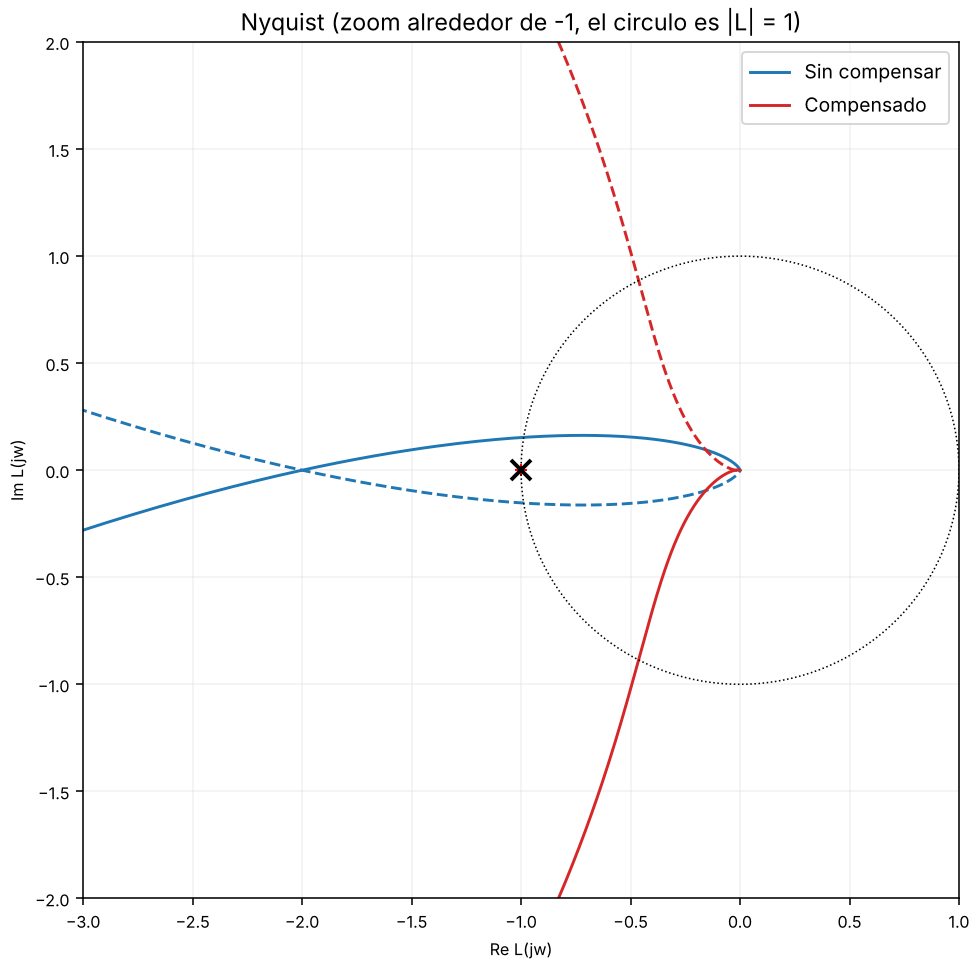
\includegraphics[width=0.49\textwidth]{figuras/p1_nyquist.png}\hfill
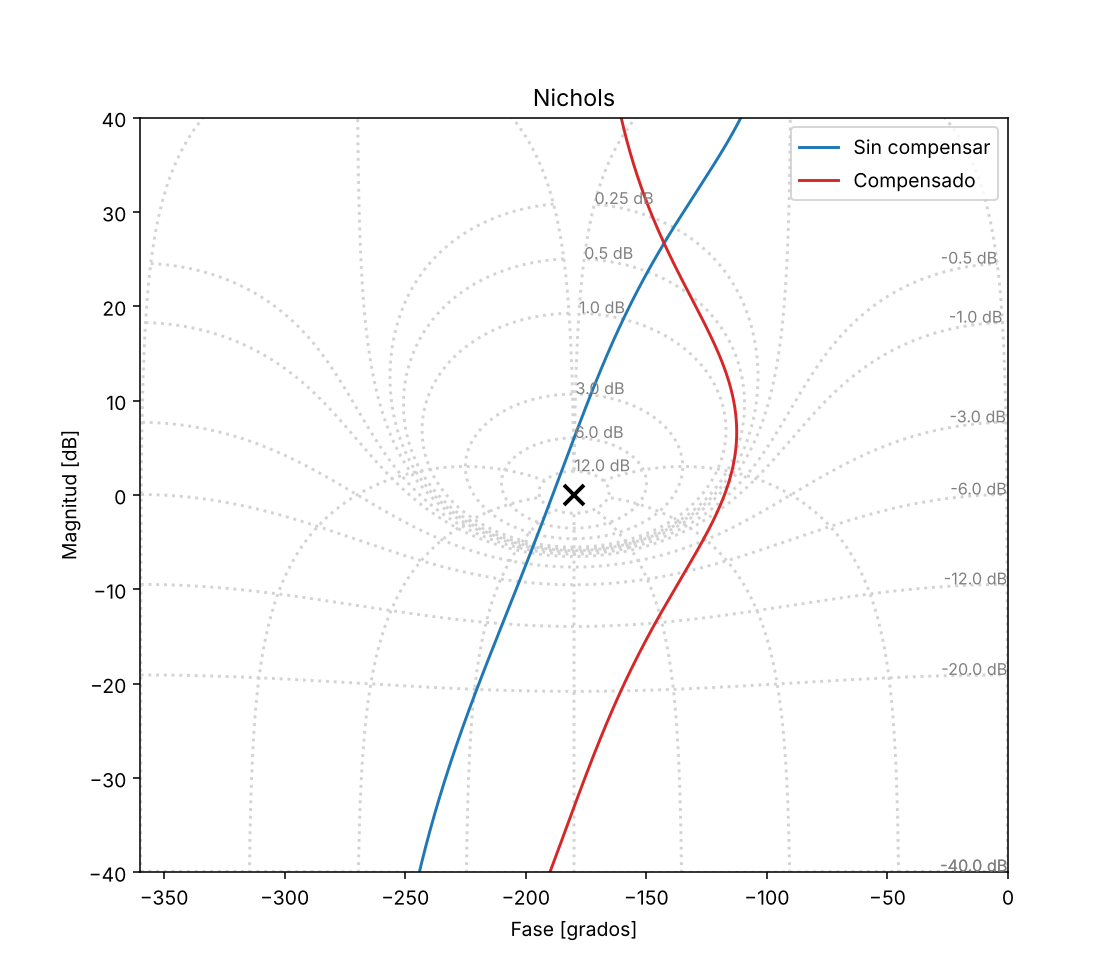
\includegraphics[width=0.49\textwidth]{figuras/p1_nichols.png}
\caption{Ejemplo A. Izquierda, Nyquist; derecha, Nichols.}
\end{figure}

En el \textbf{Nyquist}, la curva azul corta el eje real negativo en $-2$ (a la izquierda de $-1$, que es $1/\MG$): $N=2$,
$P=0$, $Z=2$, y las raíces del lazo cerrado confirman dos polos inestables ($0{,}22\pm j3{,}09$). La frecuencia de esos polos
($3{,}09\rads$) es casi la $\wc$ que leíste en el Bode: eso es lo que se ve en la oscilación creciente del escalón.
La curva roja, en cambio, queda toda dentro de la zona derecha del $-1$ y corta el círculo $|L|=1$ con mucha holgura.

En el \textbf{Nichols}, la azul cruza la línea de 0 dB en $-189^\circ$ (a la \emph{izquierda} del punto crítico) y cruza
$-180^\circ$ por encima de 0 dB: del lado inestable. La roja pasa a la derecha y por debajo del punto crítico, y roza la
curva gris de $0{,}5$--$1\dB$ (el programa da $\Mr=0{,}74\dB$).

\textbf{Compensado} (rojo). El atraso bajó la ganancia en alta frecuencia: $\wc$ cayó de $3{,}14$ a $0{,}20\rads$ y en ese cruce
la fase es $-117{,}6^\circ$, o sea $\MF=62{,}4^\circ$. $\MG$ pasó a $33{,}1\dB$. Se pagó con velocidad: el ancho de banda bajó de $4{,}67$ a
$0{,}32\rads$ y $t_s=82\,$s. La regla de segundo orden daría $M_p\approx 7\%$ para $62^\circ$; en la realidad es $11\%$,
con la cola lenta que se ve en el escalón (un polo de lazo cerrado en $-0{,}022$, casi cancelado por el cero del atraso).

\fig{p1_compensador.png}{0.6}{Ejemplo A: Bode del compensador $(50s+1)/(4700s+1)$. Cero en $0{,}02\rads$ y polo en $0{,}0002\rads$ (fuera del dibujo). En $\wc=0{,}2\rads$ resta apenas $5{,}6^\circ$.}

El compensador tiene el cero una década por debajo del nuevo cruce ($0{,}02$ contra $0{,}2$): de ahí que casi no reste fase
justo donde se mide el $\MF$ (solo $5{,}6^\circ$). Esa es la regla de diseño del atraso.

\section{Ejemplo B comentado: adelanto}

$G=10/[s(s+1)(0{,}05s+1)]$ ($K_v=10$); pedido $\MF=45^\circ$, $\MG\ge10\dB$. El programa propone
$G_c=(0{,}521s+1)/(0{,}0782s+1)$: $\alpha=0{,}150$, $\omega_m=4{,}95\rads$, cero en $1{,}92$ y polo en $12{,}8\rads$.

\begin{figure}[htbp]
\centering
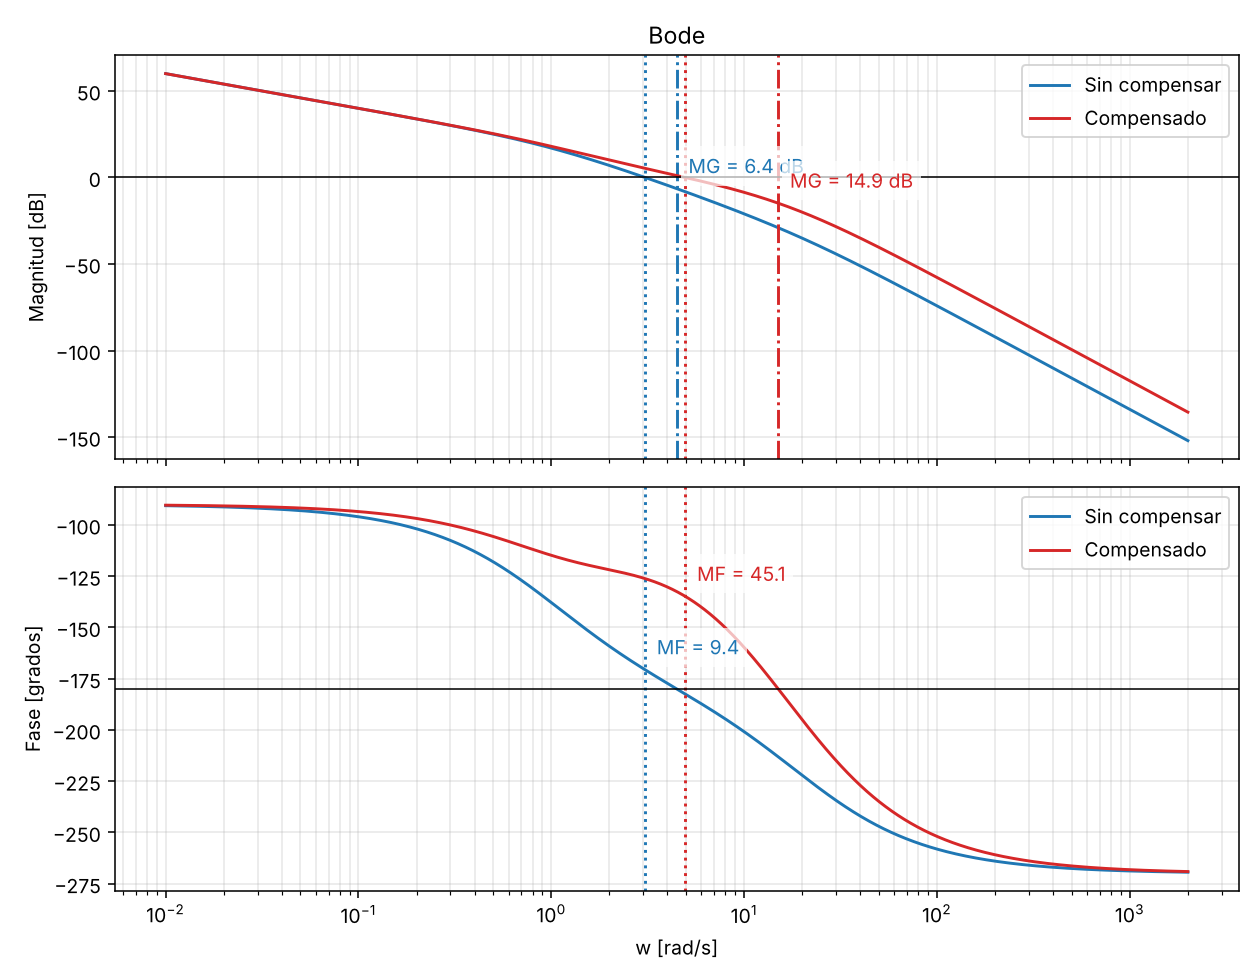
\includegraphics[width=0.49\textwidth]{figuras/lead_bode.png}\hfill
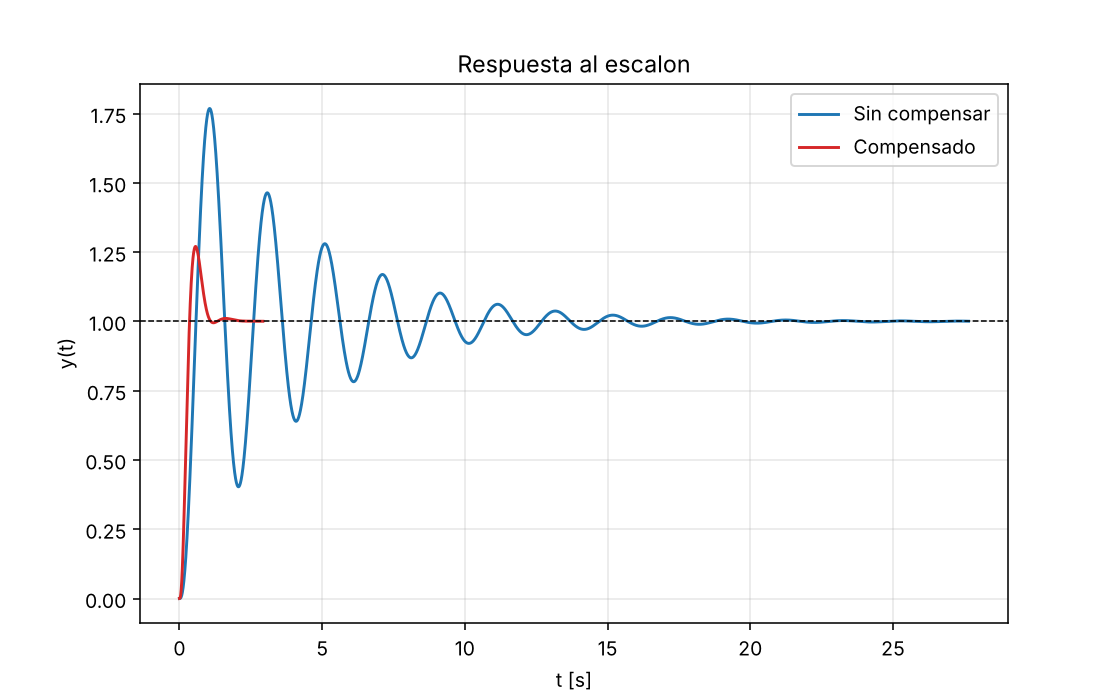
\includegraphics[width=0.49\textwidth]{figuras/lead_escalon.png}
\caption{Ejemplo B. Izquierda, Bode; derecha, escalón.}
\end{figure}

\begin{center}
\small
\begin{tabular}{@{}lrr@{}}
\toprule
& Sin compensar & Con adelanto \\
\midrule
$\MF$ & $9{,}4^\circ$ & $45{,}1^\circ$\\
$\MG$ & $6{,}4\dB$ & $14{,}9\dB$\\
$\wc$ [rad/s] & 3,07 & 4,96\\
$\Mr$ [dB] & 15,9 & 2,3\\
Ancho de banda [rad/s] & 4,8 & 9,0\\
$M_p$ & 77\,\% & 27\,\%\\
$t_s$ [s] & 15,3 & 1,0\\
\bottomrule
\end{tabular}
\end{center}

Lo que se ve: el adelanto \emph{subió} $\wc$ (más rápido) y puso una joroba de fase justo en el cruce, por eso el $\MF$ pasa de $9^\circ$
a $45^\circ$ y la oscilación se amortigua. El $\Mr=2{,}3\dB$ coincide con la cota $1/(2\sin(\MF/2))=2{,}3\dB$ de la regla de
Nichols. El costo es la ganancia de alta frecuencia: arriba del polo, el compensador multiplica por $1/\alpha=6{,}7$ ($16{,}5\dB$), y
si hay ruido de medición, se amplifica.

\section{Tabla de síntomas}

\begin{center}
\small
\begin{tabularx}{\textwidth}{@{}>{\raggedright\arraybackslash}p{3.6cm}>{\raggedright\arraybackslash}X>{\raggedright\arraybackslash}X@{}}
\toprule
Lo que ves & Qué lo explica & Qué hacer\\
\midrule
Escalón muy oscilatorio, $M_p$ alto & $\MF$ chico, $\Mr$ alto; en Nichols la curva roza una gris alta & subir el $\MF$: adelanto, o bajar $K$ \\
Escalón lento ($t_s$ grande) & $\wc$ y ancho de banda chicos & subir $K$ o usar adelanto; un atraso es lento por diseño \\
Error en régimen grande & constante de error chica (la curva baja a baja frecuencia) & subir $K$ si el $\MF$ aguanta; si no, atraso (sube la ganancia en baja sin mover $\wc$) \\
Inestable & $\MF<0$ o $\MG<1$; en Nyquist $N>0$ con $P=0$ & bajar $K$ o compensar \\
Estable pero con $\MG$ menor que 6 dB & el cruce de $-180^\circ$ está pegado al de 0 dB & bajar la ganancia de alta frecuencia: atraso \\
Escalón con cola lenta & polo y cero muy cercanos en lazo cerrado (típico de un atraso) & subir el cero del atraso (menor razón $T\wc$) si el $\MF$ lo permite \\
Mucho ruido en la salida & ganancia de alta frecuencia grande (adelanto con $\alpha$ chico) & adelanto menos agresivo o filtro \\
Cruce con pendiente $-40$ o $-60\dBdec$ & fase cerca de $-180^\circ$ o peor en $\wc$ & bajar $K$ hasta que el cruce caiga en $-20\dBdec$ o agregar adelanto \\
\bottomrule
\end{tabularx}
\end{center}

\section{Trampas al leer}

\begin{enumerate}
\item \textbf{Confundir veces con dB.} $\MG=2$ es $6{,}02\dB$; $\MG=10$ es $20\dB$. El programa imprime las dos.
\item \textbf{Lazo abierto inestable o con retardo.} El signo del margen ya no dice si el lazo cerrado es estable. Ejemplo:
 $L=2(s+3)/[s(s-1)]$ tiene $\MF=22{,}9^\circ$ y $\MG=0{,}5$ ($-6\dB$) y sin embargo el lazo cerrado es \emph{estable}
 (figura (d) del Nyquist). Hay que usar $Z=N+P$.
\item \textbf{Mirar solo el zoom del Nyquist.} Una curva que ``no se ve cerca del $-1$'' puede estar rodeándolo desde lejos;
 la cuenta $N$ del programa es la que vale.
\item \textbf{$\Mr$ no es $\MG$.} $\Mr$ es el pico de $|T|$ en lazo \emph{cerrado}; los márgenes son del lazo abierto.
 Se relacionan (ver Nichols), pero no son lo mismo.
\item \textbf{La fase del Nichols puede ``dar la vuelta''.} El eje horizontal es un ángulo: un sistema de tipo 2 empieza en
 $-180^\circ$ y baja de ahí; el programa desenrolla la fase empezando en $-90^\circ\times$tipo para que no haya saltos de $360^\circ$.
\item \textbf{Las fórmulas $\MF\approx100\zeta$ y $M_p(\zeta)$} son de segundo orden. Sirven para orientarse, no para
 informar.
\item \textbf{Bode del atraso.} Ver la nota de la sección del compensador: la curva compensada parece más baja a baja
 frecuencia pero la constante de error no cambió.
\item \textbf{Aproximar el retardo.} Para el lazo cerrado el programa usa una aproximación de Padé de orden 8; el $\MF$ y el
 Nyquist del retardo son los exactos pero el escalón es aproximado.
\end{enumerate}

\section{Fórmulas de bolsillo}

\begin{center}
\small
\renewcommand{\arraystretch}{1.35}
\begin{tabularx}{\textwidth}{@{}>{\raggedright\arraybackslash}p{4.4cm}X@{}}
\toprule
Margen de fase & $\MF=180^\circ+\angle L(j\wc)$, con $|L(j\wc)|=1$\\
Margen de ganancia & $\MG=1/|L(j\wcien)|$, $\MG_{\mathrm{dB}}=-20\log|L(j\wcien)|$, con $\angle L(j\wcien)=-180^\circ$\\
Criterio de Nyquist & $Z=N+P$ ($N$ horario); estable $\iff Z=0$\\
Cruce en Nyquist & el corte con el eje real negativo es $-1/\MG$\\
Piso de $\Mr$ por el margen de fase & $\Mr\ge 1/(2\sin(\MF/2))$\\
Segundo orden & $\MF\approx100\,\zeta$ (válido hasta $\zeta\approx0{,}6$); $\Mr=1/(2\zeta\sqrt{1-\zeta^2})$; $M_p=100e^{-\pi\zeta/\sqrt{1-\zeta^2}}$\,\%\\
Constantes de error & $K_p=L(0)$ (tipo 0); $K_v=\lim sL$ (tipo 1); $K_a=\lim s^2L$ (tipo 2). $e_{ss}$: $\frac1{1+K_p}$, $\frac1{K_v}$, $\frac1{K_a}$\\
En el Bode & tipo 1: la asíntota de $-20\dBdec$ corta 0 dB en $\omega=K_v$; tipo 2: la de $-40\dBdec$ en $\omega=\sqrt{K_a}$\\
Adelanto & $\varphi_m=\arcsin\frac{1-\alpha}{1+\alpha}$, $\alpha=\frac{1-\sin\varphi_m}{1+\sin\varphi_m}$, $\omega_m=\frac1{T\sqrt\alpha}$, ganancia en $\omega_m$: $10\log(1/\alpha)$ dB\\
Atraso & $\beta=|L(j\wc')|$ en el nuevo cruce $\wc'$; $T=10/\wc'$; en alta frecuencia baja $20\log\beta$ dB\\
Ancho de banda & aproximadamente entre 1 y 2 veces $\wc$\\
\bottomrule
\end{tabularx}
\end{center}

\end{document}
